\documentclass[a4paper, 12pt]{article}
% \documentclass[conference]{IEEEtran}

% geometry
\usepackage[top=0.5in]{geometry}
\usepackage[english]{babel}
\usepackage{pifont}
\usepackage{graphicx}
% \usepackage{blindtext}
\usepackage{float}

\usepackage[
    %backend=biber, 
    natbib=true,
    style=numeric,
    sorting=none
]{biblatex}
\addbibresource{export.bib}
\usepackage{csquotes}
\graphicspath{{./images/}}

\begin{document}
\title{\Large{\textbf{A research on using cost-effective close-range photogrammetry to digitize Rwanda's cultural heritage: A DSLR and smartphone dependent solution.}}}
\author{By Jean Nshuti \\ jnshuti@andrew.cmu.edu \\ Carnegie Mellon University — School of Engineering}
\date{\today}
\maketitle

% \textbf{\textit{Abstract} — The research investigates the necessity to have cultural tools digitized by inspecting existing methods
%     and technologies used in the sector of assets digitization. The research will spectate the effect of cultural assets' destruction on the society
%     and course of actions used to prevent that. The paper then focuses on practical considerations and presenting an overview of the technicalities using photogrammetry. \\}

% Abstract
\textbf{\textit{Abstract} — Digital cultural-heritage preservation is of a high importance but requires high resolution 3D imagery as output, yet the equipment used to generate that output, like a terrestrial laser scanner, cost between \$15,000 and \$200,000. The research then analyzes how using calibrated cost-effective close-range photogrammetry would still deliver outstanding results. The paper focuses on practical considerations and presenting an overview of the technicalities using cost-effective close range photogrammetry to preserve Rwanda's cultural heritage. \\}

\textbf{\textit{Keywords — cultural assets, cultural heritage artifacts, photogrammetry, digitization, close-range, cost-effective}}

\section{\textbf{Introduction}}
The use of photogrammetry has been on the rise since its inception some 150 years ago \cite{histphtgm}. It has been adopted by a wide range of users in fields
like research, engineering, architecture, archaeology, geology, etc.
The  American Society for Photogrammetry and Remote Sensing defined photogrammetry as \cite{Ebert2015} “the art, science, and technology
of obtaining reliable information about physical objects and the environment, through processes of recording, measuring,
and interpreting imagery and digital representations of energy patterns derived from noncontact sensor systems”. Where close-range photogrammetry or CRP is photogrammetric data collection and processing where the object is less than 300 away \cite{crp}. \\

The very rich historical background of Rwanda can be attributed to the large number of cultural assets she possesses. These assets are considered valuable and
delicate since damage of any form devalues their worth and makes it difficult to replicate or reconstruct. Total annihilation of these assets in case of misfortunes
could likely erase of trace of their existence from history. As such, digitizing such assets will preserve their existence even if they end up being destroyed. \\

A technology that captures qualitative information like texture, color and refractive index of assets has to be used. This technology will ensure that features
of these assets are capture to a higher degree of precision before being stored digitally \cite{Linder2006}. This will help when
the asset is being stored digitally to reduce the margin of error and increase accuracy \cite{accphtgm}. With this, photogrammetry can be used to further
investigate how useful it would be in digitizing Rwanda's cultural assets. \\

Since photogrammetry's foundation is based on pictures, they will be taken, processed and then digitized to produce 3D objects/assets that are cleaned and retopologized in
a 3D application. \\

As technology advances, photogrammetry becomes more user-friendly. So, using a reconstruction software
would be more effective with an expectation of reducing the loss due to machine learning. In addition, using a high-end smartphone for sampling, would produce 3D scans that can be used for testing while using a DSLR (digital single-lens reflex) camera would produce high resolution 3D scans for the final 3D asset. Gathering several pictures of different assets from museums will be the quickest way to obtain data. By comparing the digitized
asset and the real (physical) asset, we will be able to analyze and have a viable conclusion. This will result in accurate and clean assets that will
hold every data needed in digitization using a low-cost solution. \\

% Hence, this research aims at investigating the need to preserve cultural heritage and suggesting proved methods and ways to conduct a digitization of cultural heritage using
% photogrammetry in Rwanda.
Hence, this research shows how fine-tuned, cost-effective smartphone and DSLR camera could produce high resolution 3D scans in a close-range photogrammetry in comparison to high-tech, more high-priced terrestrial laser-scanner in an attempt to digitize Rwanda's culture heritage.

\section{\textbf{Literature Review}}
Cultural assets (heritage materials) are as essential as the culture itself, as they hold the meaning and history of a place.
It is the physical and intangible characteristics of civilization that have been passed down through the centuries \cite{WILLIS2014145}. For cultural assets hold a heritage
and are irreplaceable, their demise would create a gap in one nation's history hence impossible to pass the culture down.
So, the need to digitally preserve/conserve the heritage removes the unbearable effects. Yet, the usual generation of cultural heritage 3D scans requires high-priced equipment (like LiDAR scanner and laser-scanning) \cite{priced} to generate high resolution scans.\\

% An unexpected destruction to any of the artifacts would not only result in cultural deficiency but in an economic deficit as well. For instance, in 2016, New Delhi’s
% National Museum of Natural History was caught on fire where a 160 million old fossils and staffed animals were annihilated \cite{delhi012}. For that reason, digital preservation should
% be of immense interest to the nation of Rwanda. \\

The high-priced equipment were effective when the technology was in its infancy, where in some occasion, they were an overengineered solution to less complex task. This resulted in slow implementation and adoption in areas where the technology was needed \cite{ptn}. Notably, it's a costly method with limits in terms of augmenting or replacing image-based output. \\

As technology advanced, the high-priced tech was incorporated into smaller, less-priced devices. For instance, the old high-priced LiDAR technology is now a built-in feature in new iPhone smartphones, with some apps having reconstruction algorithms, the smartphone can now perform low-end photogrammetry. In addition, DSLR cameras now come with advanced image enhancing features like autofocus, light sensitivity, flash and natural daylight etc. which are useful in image scanning. Also, \cite{ptn} shows that 3D distress identification and modeling with improved spatial accuracy and automation, while keeping 2D color and shading information for data fusion from a DSLR camera, has a lot of promise. Hence, leveraging the 2 cost-effective solutions would still generate high resolution 3D scans of Rwanda's cultural heritage.

\subsection{\textbf{The History of cultural heritage digitization}}
The act of cultural assets protection/conservation started in the early 18th century, where an Austrian ruler called Maria Theresa set regulations about their protection in times of war \cite{germ72}.
But the term "cultural heritage" was adopted in November 1972 in a General Conference of UNESCO \cite{batisse01}, which indicated the benefits of protecting the unique, invaluable assets to everyone.
In the 19th \& 20th centuries, scholars felt a need to create collections of their researches after the WWII, which institutions used attract more scholars \cite{Note2011}. It was not until October 2003 when UNESCO developed a
"Charter on the Preservation of Digital Heritage", which held principles it needed to follow in order to preserve digital heritage of various assets such as
books, monuments, etc., thus the beginning and need to preserve and share the knowledge \cite{charter002}. \\

\subsection{\textbf{Methods used in cultural heritage digitization}}
The basis of cultural heritage digitization is on 2D and 3D archiving, which results in either 2D photographs or 3D models. The earliest an dsimplest form of digitization was images taken with care and stored in
museum galleries. For example, in the 1940s, The Museum of Modern Art inaugurate its photography department and George Eastman House International Museum of Photography and Film was
opened for this matter \cite{Note2011}. But as technology advances, 2 methods were invented, namely, photogrammetry and laser-scanning \cite{dgpht}. Photogrammetry which uses an \textit{image-based modelling} approach has a merit of
generating quick and effective data processing to the building of an asset. For instance, the method was utilized in China to restore  Emperor Qin’s mausoleum \cite{Zhou2012}. Companionably, laser-scanning uses \textit{range-based modelling}
which permits for the acquisition of numerous minor geometric information of an asset hence providing better precision \cite{dgpht} but with a drawback of slow data capturing, and need a multitude of manpower and resource \cite{Zhou2012}.
Regardless, the latter in parallel with other technologies was used to scan Tang Paradise \cite{dgpht}.

% \subsection{\textbf{The impact of cultural heritage digitization}}
% The eradication of heritage in any form disempowers any nation's heritage. Access to the digital heritage would create more chances for people to create, communicate and share knowledge \cite{charter002}. Additionally, virtual tours
% which is the use of 360\textsuperscript{0} videos or VR (virtual reality) to tour/explore a certain place virtually, can benefit from these assets and facilitate the sector of tourism. Notably, in the 1990s, Williams and Hobson, predicted
% that tourism was about to enter the age of VR and be used to promote tourism \cite{Yang2021}. Hence, the digitized heritage would immensely support that shift in Rwanda, in case applied. Additionally, digital education with cultural heritage
% would be facilitated by the digitized assets. For instance, in the Netherlands, during the COVID-19 pandemic \cite{eddig}, teachers, cultural heritage professionals, researchers worked with Europeana and European Schoolnet to create
% digital heritage to better integrate it in education. This end result was that 17,000 students and more benefited from this and in the proved to augment abilities in the areas of cognition, social interaction, and culture.  With the help of
% Rwanda Cultural Heritage Agency, this technology could not only aid students but commoners as well, in case the physical access to assets is restricted due an uncertainty. \\

\subsection{\textbf{The role of cost-effective equipment}}
The adoption of cost-effective equipment would benefit in the process of data collection by facilitating a low-cost close range photogrammetry since most tangible assets require a close-range image acquisition i.e. not more than 300 metres away from the device taking images \cite{cls_ran}. The whole digitization process is costly and goes through various phases, each bringing its own difficulties. Therefore, the usage of cost-effective tools to take 3D scans, would immensely save money that can be used in following phases.

\section{\textbf{Methodology}}
\subsection{Approach}
% This research paper attempts to investigate the necessity to cultural digitize heritage and suggest an effective way to carry that task using photogrammetry in Rwanda. To understand the necessity in digitizing the assets, observation through museums and places holding cultural heritage in Rwanda, was used. Whereas a considerable search on the web was used to find the effective method that might carry this task. Since cultural assets are stored in open places and that other related researches were made around this area, it was unchallenging to acquire the data. Using this data, we will demonstrate the necessity and analytical steps/methods that could be utilized.

This research paper demonstrates how the adoption of cost-effective tools in a close-range photogrammetry delivers astounding 3D scans if the settings are calibrated, in place of high-price tools that are overengineered to less complex task, in digitizing Rwanda's cultural assets. To understand how the process of delivery is done, images (data) were collected either using a high-end smartphone or a DSLR camera and occasionally extensive search on the internet. The efficient delivery then requires steps such as smartphone and DSLR camera settings, how images are acquired, ways employed to generate a 3D model, reducing the model's size by retopology or compression and how the resulting model is evaluated.

% \subsection{The necessity}
% The only known way Rwanda conserves its heritage is mostly through oral history if it is intangible \cite{unescorw}. Or taking pictures of those that are tangible but some of them were crafted very long time ago, yet very few know how to replicate or reconstruct in case one is damaged. On top of that, there is a total of 530 sites holding Rwanda's cultural and 107 of them have been extensively explored according to Rwanda Cultural Heritage Association \cite{rcha}. However, there is no structured way of conserving any of the tangible heritage.

\subsection{Smartphone and DSLR camera settings}
The replacement of high-priced with cost-effective tools if not calibrated to the best settings would be of lesser use. This is due to how high-priced tools come with specific built-in photogrammetry related features to ease the process. For instance, \cite{Geo3D2019} Teledyne Optech devices come with advanced LiDAR and camera survey features for airborne, mobile and terrestrial mapping yet at a starting price of \$65,000. By choosing a smartphone, like the latest iPhone device, the environment has to be well lit, having with softer shadows since harder shadows are recorded with a 3D scan and cannot be removed in preprocessing (model generation). The setting will then improve image quality during image acquisition. On the other side, if a DSLR is used, \cite{calib} zooming to one setting and locking it down, a 100-200 ISO range, white balance, an aperture between f8 and f11, etc. are required during the calibration process to generate images of high quality that still hold textures of assets. Hence, the close-rage image acquisition using aforementioned cost-effective devices, delivers high resolution 3D scans if settings are calibrated.

\subsection{Image acquisition}
Image acquisition in photogrammetric measuring scheme is the foundation of every other preceding step. If a stage is perfectly configured, the generated results are outstanding hence facilitating a transition to next phases. There are advanced and bigger tools for acquisition depending on how much 3D model accuracy is need according to the surface structure of the asset or how big the asset is\cite{Na2022}. For Rwanda's cultural tangible assets, a smartphone would be effective if the assets are small \cite{An2022} and an SLR (Single Lens Reflex) camera if the assets are larger \cite{cam1}. Additionally, because of technological advances, the result from the 2 gadgets mentioned, is as good as old ones made specifically for the science yet bigger and more expensive. Thus, this is considered as the main data collection method.

\subsection{Model construction}
After the acquisition, the minimum number of images requires is 50, which might aid in building a low resolution sample. There are several commercial and free reconstruction pieces of software such as Meshroom, AgiSoft Metashape, 3DF Zephyr, VisualSFM, Reality Capture, where most of them use SfM. "SfM is a photogrammetric approach that use a series of images to generate a three-dimension structure of a scene based on computer vision and visual perception" \cite{Na2022}. With our case, 3DF Zephyr freemium (only 50 images) was selected for its user-friendliness and easier learning curve for sampling. Furthermore, an open-source software, Meshroom was picked aiming for its advanced features since it can be tweaked for better results after sampling.

\begin{figure}[!h]
    \centering
    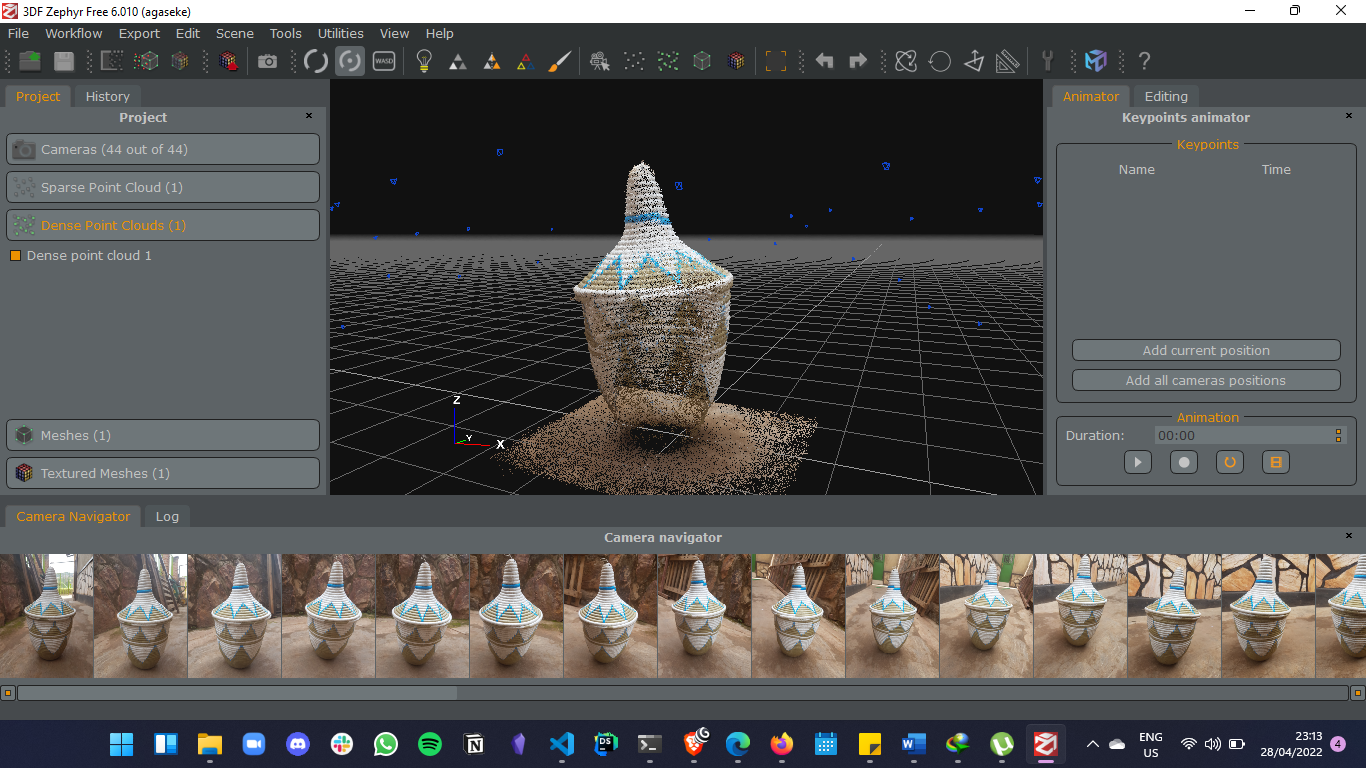
\includegraphics[width=\linewidth]{images/3df.png}
    \caption{Reconstruction in 3DF Zephyr}
    \label{fig:one}
\end{figure}

\subsection{Retopology and compression}
Model construction and extraction might look like the last phase, but the resulting model is very sizeable depending on the complexity and resolution of images acquired. For example, a small model might have more than a million faces (polygons) with 30-50 mbs \cite{Lauria2022} and occasionally the model is expected to be viewed/displayed on the web, low-end phones or smartphones. So, by using retopology which is a method of "simplifying the topology of a mesh to make it cleaner and easier to work with" \cite{reto} it would reduce its size. In addition, a lossless 3D geometric compression \cite{draco} might be added to further reach the desired size. Furthermore, this process supports the cost-effective theme since only the necessary data from a 3D model is used.

\begin{figure}[H]
    \centering
    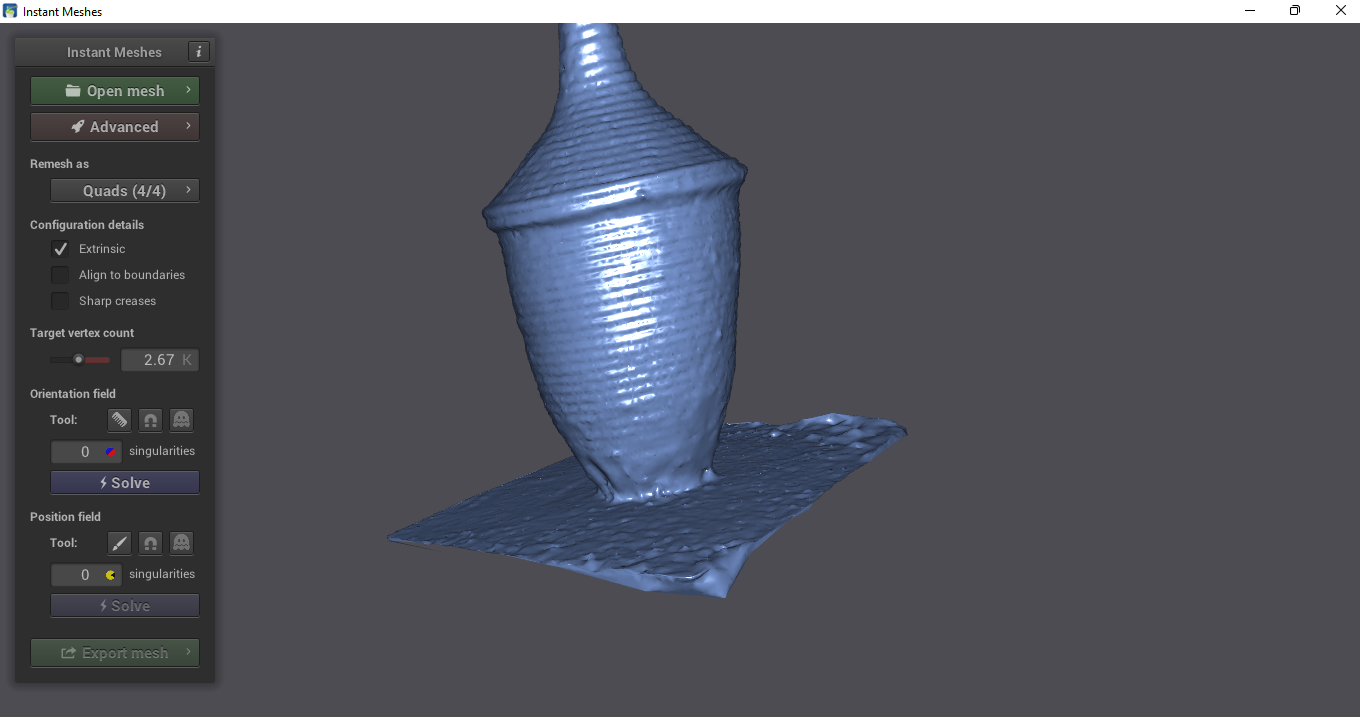
\includegraphics[width=\linewidth]{images/IM.png}
    \caption{Retopologying in Instant-Meshes}
    \label{fig:two}
\end{figure}

\subsection{Comparison and evaluation}
The measurement of the 3D model precision might be done by comparing it with physical assets \cite{An2022}. This acts as the last phase in photogrammetric reconstruction since it is when the performance of a 3D model is measured with respect to the tangible asset. For example, point-to-point distances technique can be used to investigate its geometric measurements with respect to the world \cite{article}. Textures evaluation is also an addition since the 3D model has to be identical and with enough details to look like the tangible asset texture-wise. With high-resolution images, efficiently calibrated settings, a naked eye will be enough to evaluate the similarity between both assets.

\section{\textbf{Conclusion}}
% The review investigated the history of cultural heritage digitization, methods, and the impact of digitizing cultural heritage by assessing what has been done before.
% The research showed how the need to preserve cultural assets started as early as the 18th century from an Austrian ruler during war. Even though, digitizing cultural assets started with images as soon as photographs were invented, later two
% advanced, effective methods namely laser-scanning and photogrammetry were utilized. Digitized cultural heritage impacts are several but tourism and education were found to be more closely impactful to the society. From this research it's clear
% that Rwanda as a regional ICT/Tech hub \cite{rwtechub} would leverage this technology to preserve and conserve its culture for next generations using photogrammetry. Moving forward, this research recommends effective technicalities driven by past literatures on how
% cultural heritage can be preserved in Rwanda.

The research demonstrated how the implementation of cost-effective close-range photogrammetry using calibrated settings to collect data via a high-end smartphone and a DSLR camera, would produce high resolution 3D scans without a need of installing high-priced tools. The research showed the importance of regulating settings to reach the required image quality even though tools are of a lower cost, collecting data using either a smartphone for sampling and a DSLR camera for final results, model construction in 3DF Zephyr, reducing the model's size and how to evaluate its performance. From this research, it was observed that adopting cost-effective tools in a close-range photogrammetry, would save money that might be used in further steps that are as demanding such as model construction which requires excessive use of computer memory, speed and GPU. From this research it's clear that Rwanda as a regional ICT/Tech hub \cite{rwtechub} would leverage this technology to preserve and conserve its culture for next generations using cost-effective close-range photogrammetry.

\printbibliography
\end{document}


